\section{Background and Motivation}\label{sec:motivation}

In this section, we first introduce how mechanized specifications describe the
language syntax and semantics.
%
While most existing mechanized specifications of programming languages have been
outdated, mechanized specifications of JavaScript are actively maintained.
%
The well-organized official language specification, ECMA-262~\cite{es13}, makes
it possible even though it is a real-world programming language used in diverse
fields with massive language semantics.
%
Because existing JavaScript mechanized specifications~\cite{kjs, javert, jiset,
skel-js} mimic the abstract algorithms in ECMA-262 almost as it is, we explain
the JavaScript mechanized specification using ECMA-262.
%
Then, we explain the control-flow graph (CFG) in the mechanized specification
and how to use it in coverage-guided fuzzing as an example.
%
Finally, we explain why a simple node coverage cannot fully discriminate
different semantics in different language features or even in the same features.

%----------------------------------------%
%----------------------------------------%

\subsection{JavaScript Language Specification (ECMA-262)}\label{sec:ecma-262}

Now, we explain how the latest version of ECAM-262 (ES13, 2022) describes
JavaScript syntax and semantics of language features with simple examples. 

%----------------------------------------%
%----------------------------------------%

\subsubsection{Syntax}\label{sec:syntax}

\begin{figure}
  \centering
  \begin{subfigure}{\textwidth}
    \[
      \small
      \begin{array}{l}
        \esntp{AdditiveExpression}{Yield, Await} \est{:}\\

        \qquad \esntp{MultiplicativeExpression}{?Yield, ?Await}\\

        \qquad \esntp{AdditiveExpression}{?Yield, ?Await} \; \est{+} \;
        \esntp{MultiplicativeExpression}{?Yield, ?Await}\\

        \qquad \esntp{AdditiveExpression}{?Yield, ?Await} \; \est{-} \;
        \esntp{MultiplicativeExpression}{?Yield, ?Await}\\
      \end{array}
    \]
  \end{subfigure}
  \caption{
    The syntax of \esnt{AdditiveExpression} in ES13.
  }
  \label{fig:add-syntax}
\end{figure}

JavaScript syntax is defined with a variant of the extended Backus–Naur form
(EBNF).
%
It consists of syntactic productions defined with multiple alternatives, and
each alternative is a sequence of symbols.
%
Unlike the original EBNF, its nonterminals are parametric with boolean
arguments; $\esparam{?}$ denotes passing the argument as is, and $\esparam{+}$
and $\esparam{\(\sim\)}$ denote passing the \scode{true} and \scode{false},
respectively.
%
Beyond parametric nonterminals, it even provides context-sensitive symbols,
conditional alternatives, etc.
%
For example, consider the following simple additive expression:
%
\begin{equation}\label{equ:add}
  \jscode{1 + 2}
\end{equation}
%
It tries to compute the addition of two Number values, \jscode{1} and
\jscode{2}.
%
Figure~\ref{fig:add-syntax} describes its syntax with the production of
\esnt{AdditiveExpression}.
%
It requires two boolean parameters, \esparam{Yield} and \esparam{Await}, and
consists of three alternatives.
%
The second (or third) one consists of three symbols, a nonterminal
\esnt{AdditiveExpression}, a terminal \est{+} (or \est{-}), and a nonterminal
\esnt{MultiplicativeExpression}.

%----------------------------------------%
%----------------------------------------%

\subsubsection{Semantics}\label{sec:sem}

\begin{figure}
  \centering
  \begin{subfigure}{\textwidth}
    \small
    %----------------------------------------%
    $\fbox{\textsf{Syntax-directed operations (SDOs)}}$
    \vspace*{0.5em}\\
    %----------------------------------------%
    \textbf{Evaluation} of
    \esnt{AdditiveExpression} \est{:} \esnt{AdditiveExpression} \est{+}
    \esnt{MultiplicativeExpression}
    \\
    \null\quad 1. Return ?$\lab{2}$
    \esalg{EvaluateStringOrNumericBinaryExpression}$\lab{1}$(\esnt{AdditiveExpression},
    \escode{+}, \esnt{MultiplicativeExpression}).$\lab{3}$
    \vspace*{0.5em}\\
    %----------------------------------------%
    \textbf{Evaluation} of
    \esnt{AdditiveExpression} \est{:} \esnt{AdditiveExpression} \est{-}
    \esnt{MultiplicativeExpression}
    \\
    \null\quad 1. Return ?$\lab{5}$
    \esalg{EvaluateStringOrNumericBinaryExpression}$\lab{4}$(\esnt{AdditiveExpression},
    \escode{-}, \esnt{MultiplicativeExpression}).$\lab{6}$

  \end{subfigure}
  \caption{
    The semantics of \esnt{AdditiveExpression} defined with two syntax-directed
    operations (SDOs) in ES13.
  }
  \label{fig:add-sdo}
\end{figure}

The language specification describes semantics using abstract algorithms, and
there are three different kinds of abstract algorithms:
%
\begin{itemize}
  \item Syntax-directed operations (SDOs) (e.g., \textbf{Evaluation} of
    \esnt{AdditiveExpression} \est{:} $\cdots$ in Figure~\ref{fig:add-sdo})

  \item Normal algorithms (e.g., \textbf{ToNumeric} in
    Figure~\ref{fig:normal-algos})

  \item Built-in methods (e.g., \textbf{Number} in
    Figure~\ref{fig:builtin-number})
\end{itemize}

%----------------------------------------%

A \textit{syntax-directed operation (SDO)} defines the semantics of each
alternative in syntactic productions.
%
It consists of 1) target alternative, 2) name, 3) optional parameters, and 4)
body.
%
Each algorithm body is a pseudo-code consisting of well-organized steps written
in a natural language, English.
%
For example, two abstract algorithms in Figure~\ref{fig:add-sdo} are SDOs whose
target alternatives are the second and third ones of the
\esnt{AdditiveExpression} production for addition (\scode{+}) and subtraction
(\scode{-}) operators.
%
Their names are \textbf{Evaluation} with no optional parameters, and
bodies consist of a single step that invokes another normal algorithm
\textbf{EvaluateStringOrNumericBinaryExpression}.
%
Note that the variables \esnt{AdditiveExpression} and
\esnt{MultiplicativeExpression} in these SDOs store \textit{abstract syntax
trees (ASTs)} of the left- and right-hand side of given additive expressions.
%
For instance, if the first SDO in Figure~\ref{fig:add-sdo} takes the additive
expressions in~(\ref{equ:add}), the two metavariables store ASTs of two Number
literals, \jscode{1} and \jscode{2}, respectively.
%
It means that abstract algorithms in ECMA-262 treat ASTs as values, and could
store them in variables or pass them as arguments of other algorithms.
%
The ``?'' operator is a shorthand for the following sequence of steps to handle
control flows:
\vspace*{.5em}\\
{
  \noindent
  \null\qquad 1. If \esvar{argument} is an abrupt completion, return
  \esalg{Completion}(\esvar{argument}).
  \\
  \null\qquad 2. Else if \esvar{argument} is a Completion Record, set
  \esvar{argument} to \esvar{argument}.[[Value]].
}
\vspace*{.5em}\\
where a completion record is \textit{abrupt} when it represents exceptional
control flows, such as \jscode{throw}, \jscode{return}, \jscode{break}, and
\jscode{continue}.
%
In other words, the ``?'' operator is a branch that checks whether given
values are abrupt completions and directly returns them if so.

%----------------------------------------%

\begin{figure}
  \centering
  \begin{subfigure}{\textwidth}
    \small
    %----------------------------------------%
    $\fbox{\textsf{Normal algorithms}}$
    \vspace*{0.5em}\\
    %----------------------------------------%
    \textbf{EvaluateStringOrNumericBinaryExpression} (
      \esvar{leftOperand},
      \esvar{opText},
      \esvar{rightOperand}
    )
    \\
    \null\quad $\lab{7}$...
    \\
    \null\quad 5. Return ?$\lab{9}$
    \esalg{ApplyStringOrNumericBinaryOperator}$\lab{8}$(\esvar{lval},
    \esvar{opText}, \esvar{rval}).$\lab{10}$
    \vspace*{0.5em}\\
    %----------------------------------------%
    \textbf{ApplyStringOrNumericBinaryOperator} (
      \esvar{lval},
      \esvar{opText},
      \esvar{rval}
    )
    \\
    \null\quad $\lab{11}$...
    \\
    \null\quad 3. Let \esvar{lnum} be ?$\lab{13}$
    \esalg{ToNumeric}$\lab{12}$(\esvar{lval}).
    \\
    \null\quad 4. Let \esvar{rnum} be ?$\lab{15}$
    \esalg{ToNumeric}$\lab{14}$(\esvar{rval}).
    \\
    \null\quad 5. If \esalg{Type}(\esvar{lnum}) is different from
    \esalg{Type}(\esvar{rnum})$\lab{16}$, \cfbox{red}{throw a \esval{TypeError}
    exception.}$\lab{\inred{17}}$
    \\
    \null\quad ...$\lab{18}$
    \vspace*{0.5em}\\
    %----------------------------------------%
    \textbf{ToNumeric} ( \esvar{value} )
    \\
    \null\quad $\lab{19}$...
    \\
    \null\quad 2. If \esalg{Type}(\esvar{primValue}) is BigInt$\lab{20}$,
    \cfbox{red}{return
    \esvar{primValue}.}$\lab{\inred{21}}$
    \\
    \null\quad ...$\lab{22}$
  \end{subfigure}
  \caption{Three normal algorithms transitively used in the semantics of
  \esnt{AdditiveExpression} in ES13.}
  \label{fig:normal-algos}
  \vspace*{-1em}
\end{figure}

A \textit{normal algorithm} is the primary form of an abstract algorithm defined
by its 1) name, 2) parameters, and 3) body.
%
It is commonly used as a helper function, and multiple normal algorithms are
used when defining the semantics of language features.
%
Hence, the semantics of different language features often share the same normal
algorithms.
%
For example, both SDOs in Figure~\ref{fig:add-sdo} invoke the same normal
algorithm \textbf{EvaluateStringOrNumericBinaryExpression} with different second
arguments \escode{+} and \escode{-}, respectively.
%
Then, it transitively invokes other normal algorithms,
\textbf{ApplyStringOrNumericBinaryOperator} and \textbf{ToNumeric}.
%
Thus, at least three normal algorithms are shared in the semantics of the
addition and subtraction expressions.

%----------------------------------------%

\begin{figure}
  \centering
  \begin{subfigure}{\textwidth}
    \small
    %----------------------------------------%
    $\fbox{\textsf{Built-in methods}}$
    \vspace*{0.5em}\\
    %----------------------------------------%
    \textbf{Number} ( \esvar{value} )
    \\
    \null\quad 1. If \esvar{value} is present$\lab{23}$, then
    \\
    \null\quad\quad a. Let \esvar{prim} be ?$\lab{25}$
    \esalg{ToNumeric}$\lab{24}$(\esvar{value}).
    \\
    \null\quad ...$\lab{26}$
  \end{subfigure}
  \caption{
    The built-in method \textbf{Number} in ES13.
  }
  \label{fig:builtin-number}
\end{figure}

JavaScript provides diverse built-in APIs as opaque functions, such as
\jscode{Object.getPrototypeOf} and \jscode{Number.prototype.toString}.
%
A \textit{built-in method} defines the semantics of a built-in API.
%
For example, Figure~\ref{fig:builtin-number} defines the semantics of the
\jscode{Number} built-in API.
%
Since its basic functionality is to convert a given JavaScript value to the
corresponding Number value, it utilizes the normal algorithm \textbf{ToNumeric}
as a helper fucntion as well.

%----------------------------------------%
%----------------------------------------%

\subsubsection{Language Features}\label{sec:feat}

In JavaScript, a language feature is 1) a \textit{syntactic feature} or 2) a
\textit{built-in API feature}.
%
A syntactic feature is related to specific JavaScript syntax consisting of an
alternative in a syntactic production and corresponding SDO.
%
On the other hand, a built-in API feature is related to a built-in API instead
of a specific syntax.
%
For example, the addition (\scode{+}) and subtraction (\scode{-}) operators are
syntactic features ($\addfeat$ and $\subfeat$) defined by the second and third
alternatives of \esnt{AdditiveExpression} and corresponding \textbf{Evaluation}
SDOs.
%
The \textbf{Number} built-method describes the semantics of a built-in
\jscode{Number} API feature ($\numfeat$).

%----------------------------------------%
%----------------------------------------%

\subsection{Control Flow Graph (CFG) in Mechanized Specification}\label{sec:cfg}

\begin{figure}
  \centering
  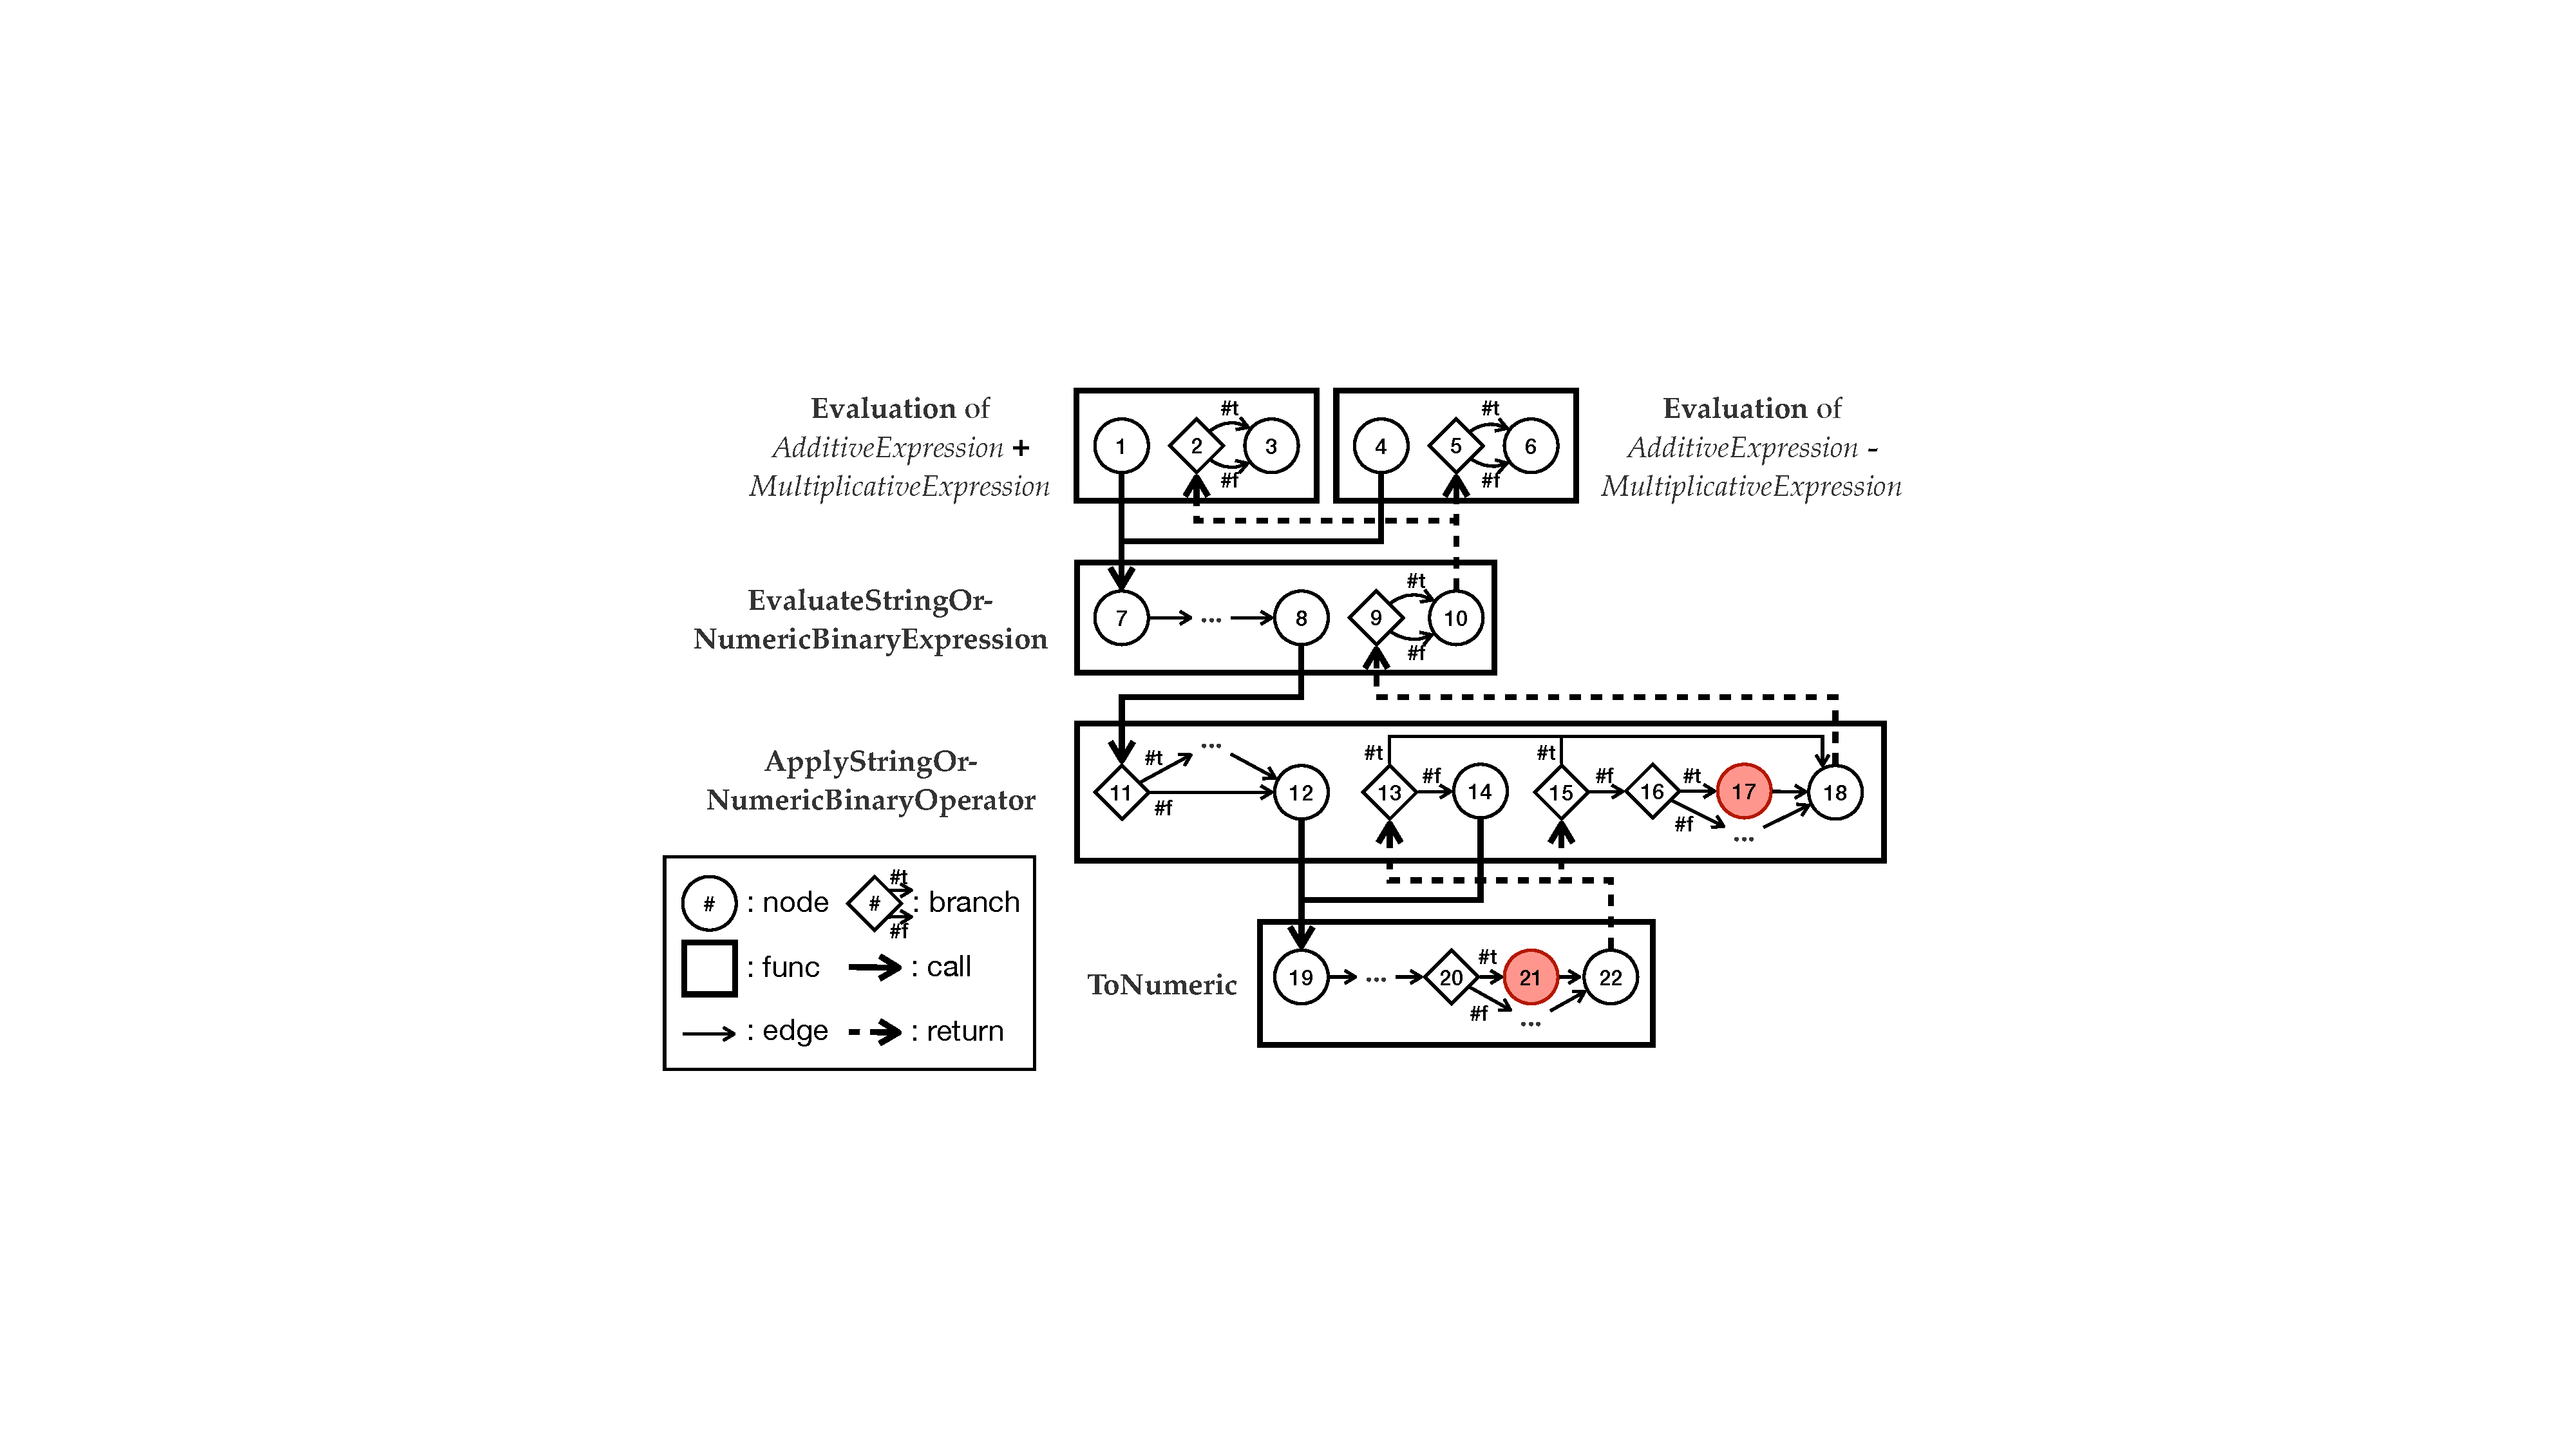
\includegraphics[width=0.85\textwidth]{img/spec-cfg}
  \caption{
    The control-flow graph (CFG) of abstract algorithms in
    Figure~\ref{fig:add-sdo}, \ref{fig:normal-algos}, and
    \ref{fig:builtin-number}.
  }
  \label{fig:spec-cfg}
\end{figure}

%----------------------------------------%

To define the coverage of a conformance test suite using the graph coverage, we
need a directed graph in the mechanized specification for JavaScript.
%
The control flow graph (CFG) is the most common way to construct a directed
graph from the JavaScript mechanized specification.
%
In the CFG, a node denotes a sequence of linear instructions, and an edge
indicates a control flow in the mechanized specification.
%
Besides, an edge often has an annotation to represent a specific control flow,
such as conditional branches (\sname{\#t} or \sname{\#f}) and function calls
(\sname{call}) and returns (\sname{ret}).

%----------------------------------------%

For example, Figure~\ref{fig:spec-cfg} depicts a CFG of the abstract algorithms
in Figures~\ref{fig:add-sdo}, \ref{fig:normal-algos}, and
\ref{fig:builtin-number}.
%
In this figure, circles (or diamonds) denote nodes (or branches), arrows denote
arrows, and boxes indicate algorithms.
%
The labels inside nodes match the labels annotated in the algorithms in
Figures~\ref{fig:add-sdo}, \ref{fig:normal-algos}, and \ref{fig:builtin-number}.
%
Now, try to apply a coverage-guided fuzzing~\cite{afl} with a node coverage
criterion in the CFG, and assume that a simple JavaScript program, \jscode{1 +
2}, exists in the program pool.
%
It does not satisfy the condition in the branch labeled 20 because the left- and
right-hand sides of \jscode{1 + 2} are both Number values rather than BigInt
values.
%
Thus, it does not cover the red node labeled 21.
%
On the other hand, another program, \jscode{3n + 4n}, is generated by mutating
the previous program.
%
Then, it now covers the red node labeled 21 because it satisfies the condition
in the branch labeled 20 with BigInt values as both sides of operands.

%----------------------------------------%
%----------------------------------------%

\subsection{Motivation}\label{sec:motiv}

Unfortunately, a simple node coverage in CFGs of mechanized specifications
cannot fully discriminate different semantics in different language features or
even in the same features.
%
We explain such cases with simple examples in the CFG depicted in
Figure~\ref{fig:spec-cfg}.

%----------------------------------------%
%----------------------------------------%

\subsubsection{Different Semantics in Different Language
Features}\label{sec:diff-feat}

The semantics of different language features might share the same abstract
algorithms as helper functions.
%
For example, the semantics of addition (\scode{+}) and subtraction (\scode{-})
operators transitively utilize the \textbf{ApplyStringOrNumericBinaryOperator}
algorithm as a helpers functions.
%
In the algorithm, the red node labeled 17 represents a semantics that throws a
\textbf{TypeError} exception.
%
If the program pool contains a program \jscode{2n + 1}, it covers the red node
labeled 17 because it has different types of numeric values, a BigInt
\jscode{2n} and a Number \jscode{1}, as the left- and right-hand sides of the
addition operator (\scode{+}).
%
Similarly, another program \jscode{2n - 1}, that uses the subtraction operator
(\scode{-}) instead of (\scode{+}), also covers the node.
%
Unfortunately, \jscode{2n - 1} would not be added to the program pool because
the node labeled 17 is already covered by \jscode{2n + 1}, while \jscode{2n - 1}
is a meaningful edge case that throws a \textbf{TypeError} exception.
%
Therefore, we need a more fine-grained definition of graph coverage criteria
that discriminates \jscode{2n + 1} and \jscode{2n - 1} for a better quality of
conformance test suite.

%----------------------------------------%
%----------------------------------------%

\subsubsection{Different Semantics in Same Language
Features}\label{sec:same-feat}

In addition, different parts in the semantics of even the same language features
might utilize the same algorithms more than once as helper functions.
%
For example, the semantics of the addition operator (\scode{+}) utilize the
\textbf{ApplyStringOrNumericBinaryOperator} algorithm, and it invokes the
\textbf{ToNumeric} algorithm twice in the nodes labeled 12 and 14.
%
Now, assume that the current program pool contains a program \jscode{2n + 1}
again.
%
Then, the red node labeled 21 is covered by the program \jscode{2n + 1} because
the left-hand side is a BigInt \jscode{2n}.
%
It means that another similar program \jscode{1 + 2n} would not be added to the
program pool because the test requirement for node labeled 21 is already covered
by \jscode{2n + 1}.
%
However, \jscode{1 + 2n} is also a meaningful test case because it checks the
edge case when the right-hand side of the addition operator (\scode{+}) is a
BigInt value.

%----------------------------------------%

In the remainder of the paper, we formally define a feature-sensitive coverage
criterion and its variants to resolve this problem (Section~\ref{sec:fscov}).
%
Then, we explain how to implement a conformance test synthesizer $\tool$ with
feature-sensitive coverage criteria in Section~\ref{sec:impl}.
%
Finally, after we evaluate feature-sensitive coverage criteria with $\tool$
(Section~\ref{sec:eval}), we discuss related work (Section~\ref{sec:related})
and conclude (Section~\ref{sec:conclusion}).
